%\documentclass[tikz, border=5pt]{standalone}
\begin{document}
	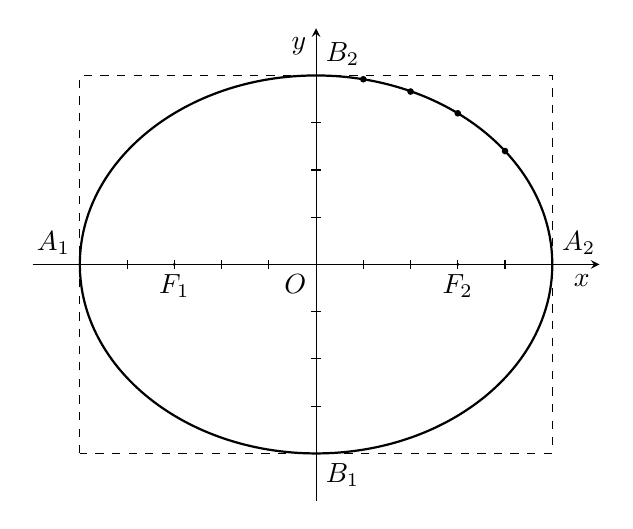
\begin{tikzpicture}[>=stealth, scale=0.6]
		% 1. 定义椭圆参数(长半轴a=5,短半轴b=4,焦距c=3,满足c=√(a²-b²))
		\def\a{5}  % 长半轴
		\def\b{4}  % 短半轴
		\def\c{3} % 焦距(近似√(5²-3²)=√16≈4)
		
		% 2. 绘制辅助矩形(虚线)
		\draw[dashed] (-\a, -\b) rectangle (\a, \b);
		
		% 3. 绘制椭圆
		\draw[thick] (0,0) ellipse ({\a} and {\b});
		
		% 4. 绘制坐标轴
		\draw[->] (-\a-1,0) -- (\a+1,0) node[below left] {$x$};
		\draw[->] (0,-\b-1) -- (0,\b+1) node[below left] {$y$};
		\node at (0,0) [below left] {$O$}; % 原点
		
		% 绘制所有小刻度线(从 -1 到 2,每隔 1 单位画竖线)
		\foreach \x in {-4,-3,...,4} {
			\draw (\x, 0.1) -- (\x, -0.1) ;  % 小竖线(长 0.2 单位)
		}
		\foreach \y in {-3,-2,...,3} {
			\draw (0.1,\y) -- (-0.1,\y) ;  % 小竖线(长 0.2 单位)
		}
		
		% 5. 标记顶点与焦点
		\node at (-\a,0) [above left] {$A_1$};   % 左顶点
		\node at (\a,0)  [above right] {$A_2$};  % 右顶点
		\node at (0,\b)  [above right] {$B_2$};  % 上顶点
		\node at (0,-\b) [below right] {$B_1$};  % 下顶点
		\fill (-\c,0) circle (1pt) node[below] {$F_1$}; % 左焦点
		\fill (\c,0) circle (1pt) node[below] {$F_2$}; % 右焦点
		
		% 6. 绘制
		\fill (1,3.92) circle(2pt);
		\fill (2,3.66) circle(2pt);
		\fill (3,3.2) circle(2pt);
		\fill (4,2.4) circle(2pt);
		
	\end{tikzpicture}
\end{document}
